\begin{appendices}
%\appendixpage
%\noappendicestocpagenum
%\addappheadtotoc
\chapter{Publications} \label{publications}
\
A. Astudillo, P. Muñoz, F. Alvarez and E. Rosero, “Altitude and attitude cascade controller for a smartphone-based quadcopter,” in \textit{2017 International Conference on Unmanned Aircraft Systems (ICUAS)}. IEEE, jun 2017, pp. 1447–1454. [Online]. Available: \url{http://ieeexplore.ieee.org/document/7991400/}
\\\\
A. Astudillo, B. Bacca and E. Rosero, “Optimal and robust controllers design for a smartphone-based quadrotor,” in \textit{2017 IEEE 3rd Colombian Conference on Automatic Control (CCAC)}
\\\\
\textbf{(Paper Submitted to Journal)} A. Astudillo, P. Muñoz and E. Rosero, “Cascade Controller for Autonomous Flight of a Smartphone-based Quadrotor,” in \textit{Journal of Intelligent \& Robotic Systems, SI: UAS-2017}.

\chapter{Supplementary Material} \label{supplementary}
\
All supplementary material including the Android app code, GCS code, Arduino code, 3D objects, etc., is hosted in:
\url{https://goo.gl/U43bB6}


\chapter{Control Signals in Flight Tests}\label{controlsignals}

\section*{Stabilize Mode}

\subsection*{LQI Controller}

\begin{figure}[H]
\begin{subfigure}{0.5\linewidth}
\centering
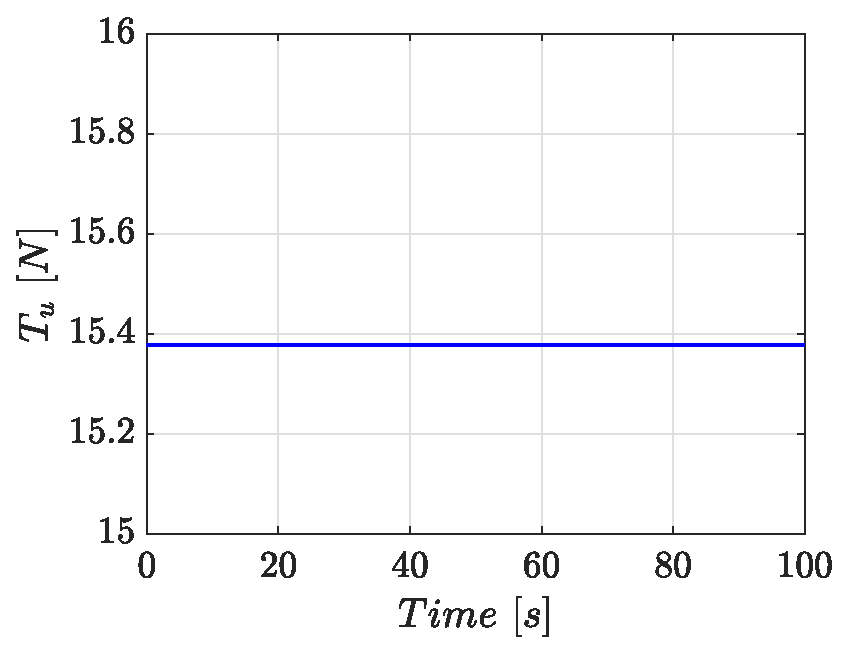
\includegraphics[width=7.0cm]{stabilize_u_lqi_imp}
\caption{Thrust}
\label{fig:stabilize_u_lqi_imp}
\end{subfigure}%
\begin{subfigure}{0.5\linewidth}
\centering
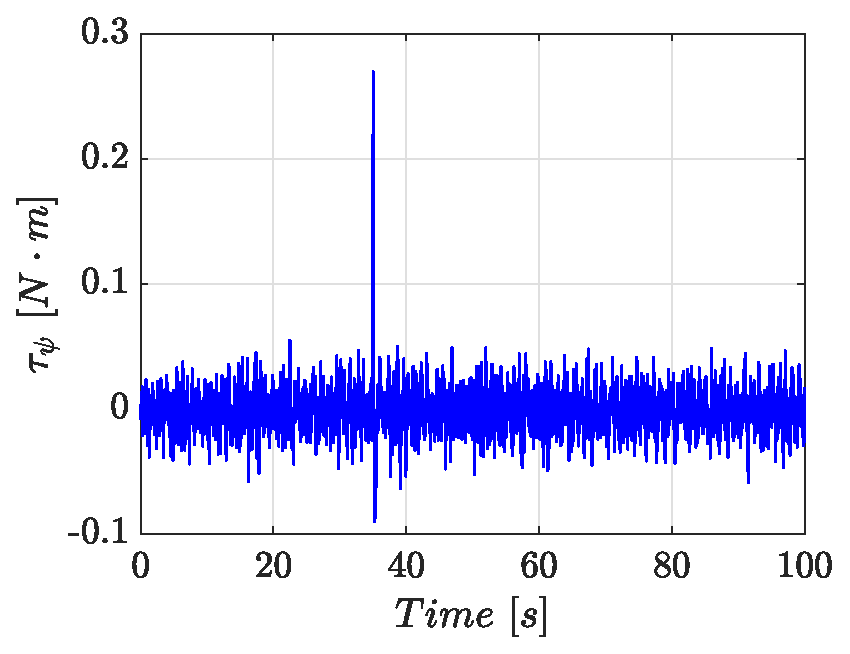
\includegraphics[width=7.0cm]{stabilize_taupsi_lqi_imp}
\caption{Yaw torque}
\label{fig:stabilize_taupsi_lqi_imp}
\end{subfigure}\\[1ex]
\begin{subfigure}{0.5\linewidth}
\centering
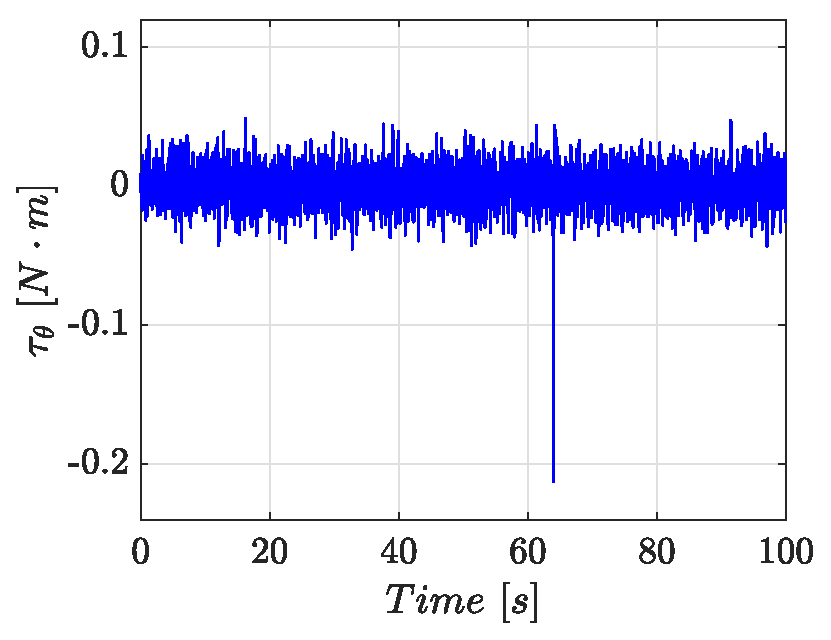
\includegraphics[width=7.0cm]{stabilize_tautheta_lqi_imp}
\caption{Roll torque}
\label{fig:stabilize_tautheta_lqi_imp}
\end{subfigure}
\begin{subfigure}{0.5\linewidth}
\centering
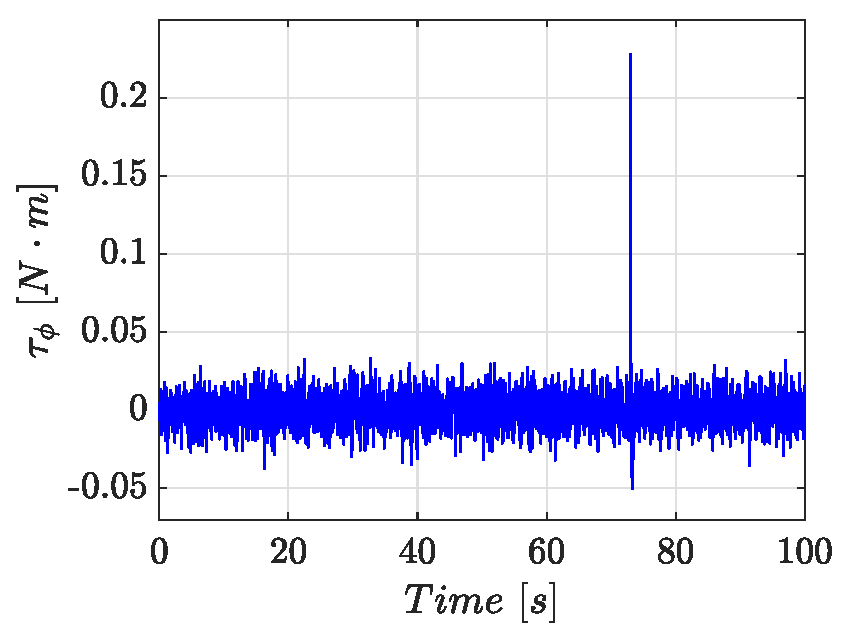
\includegraphics[width=7.0cm]{stabilize_tauphi_lqi_imp}
\caption{Pitch torque}
\label{fig:stabilize_tauphi_lqi_imp}
\end{subfigure}
\caption{Control signals in LQI control test for stabilize mode}
\label{fig:stabilize_control_lqi}
\end{figure}

\begin{figure}[H]
\begin{subfigure}{.5\linewidth}
\centering
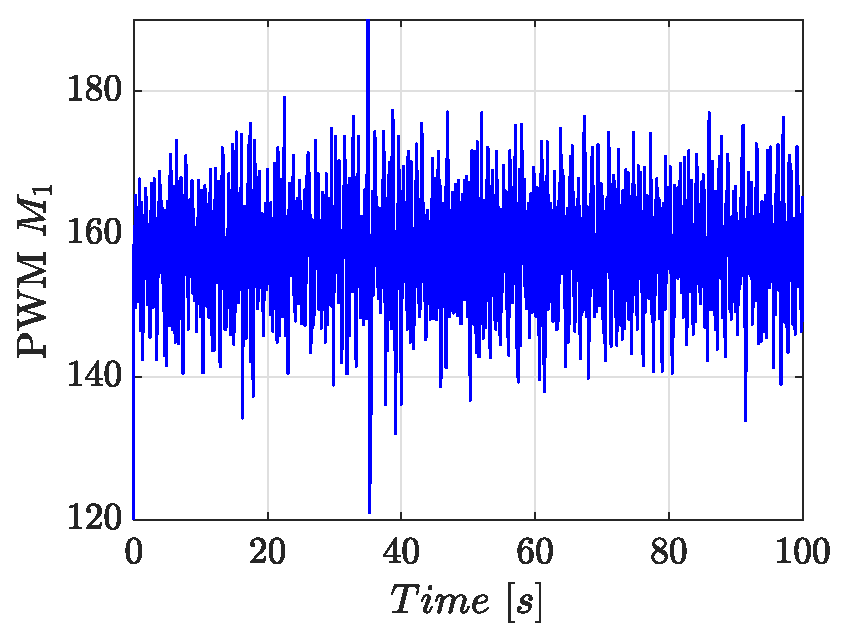
\includegraphics[width=7.0cm]{stabilize_pwm1_lqi_imp}
\caption{\textit{PWM} signal in Motor $M_1$}
\label{fig:stabilize_pwm_lqi_imp}
\end{subfigure}%
\begin{subfigure}{.5\linewidth}
\centering
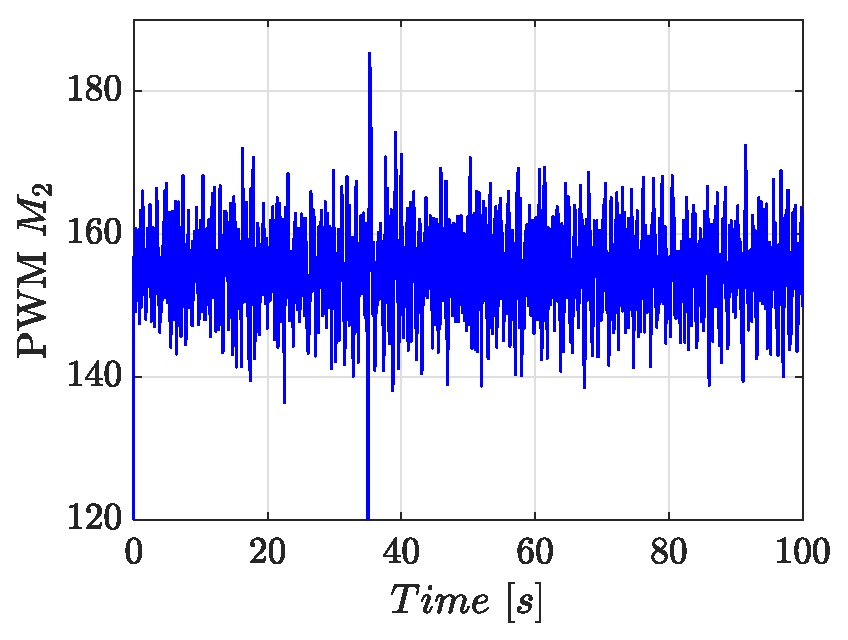
\includegraphics[width=7.0cm]{stabilize_pwm2_lqi_imp}
\caption{\textit{PWM} signal in Motor $M_2$}
\label{fig:stabilize_pwm2_lqi_imp}
\end{subfigure}\\[1ex]
\begin{subfigure}{0.5\linewidth}
\centering
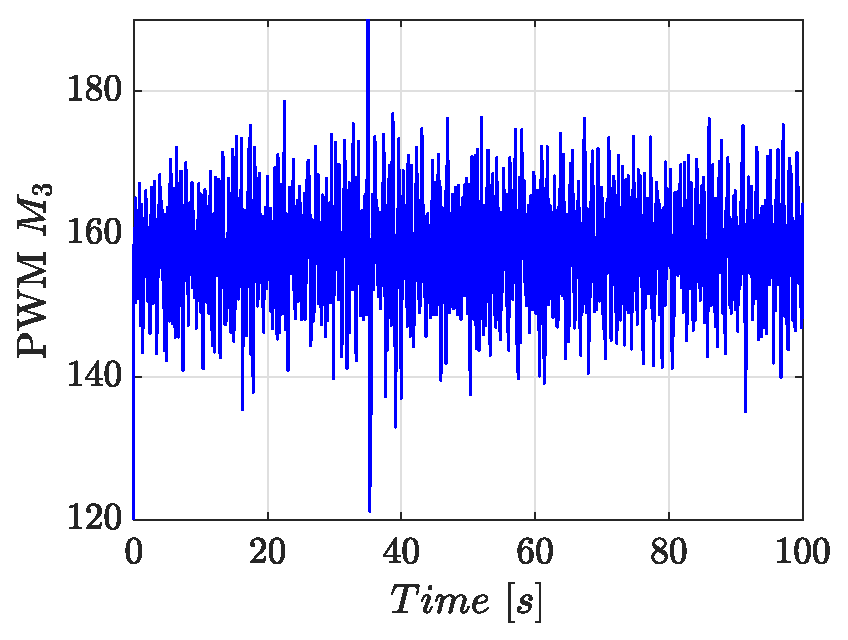
\includegraphics[width=7.0cm]{stabilize_pwm3_lqi_imp}
\caption{\textit{PWM} signal in Motor $M_3$}
\label{fig:stabilize_pwm3_lqi_imp}
\end{subfigure}
\begin{subfigure}{0.5\linewidth}
\centering
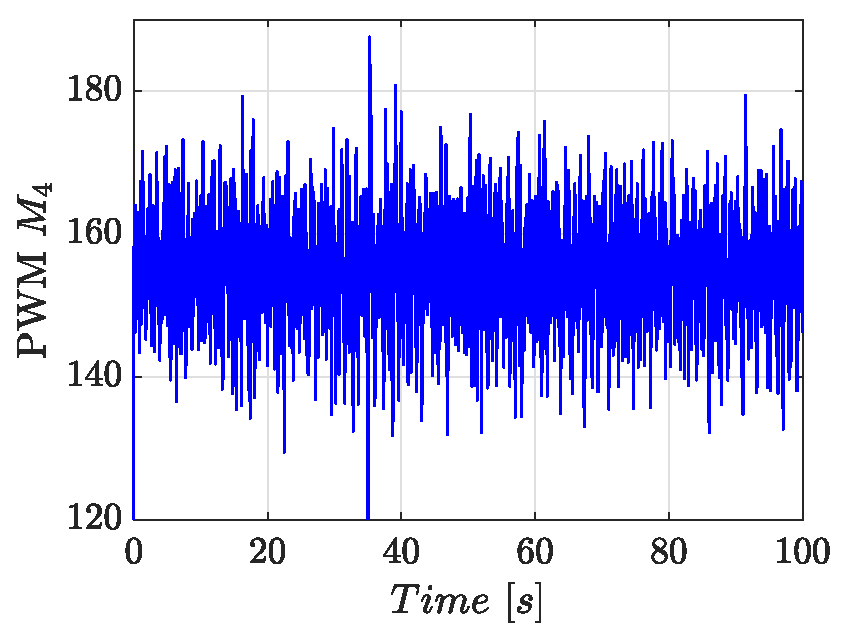
\includegraphics[width=7.0cm]{stabilize_pwm4_lqi_imp}
\caption{\textit{PWM} signal in Motor $M_4$}
\label{fig:stabilize_pwm4_lqi_imp}
\end{subfigure}
\caption{\textit{PWM} signals in LQI control test for stabilize mode}
\label{fig:stabilize_pwm_lqi}
\end{figure}

\subsection*{$H_\infty$ Controller}

\begin{figure}[H]
\begin{subfigure}{.5\linewidth}
\centering
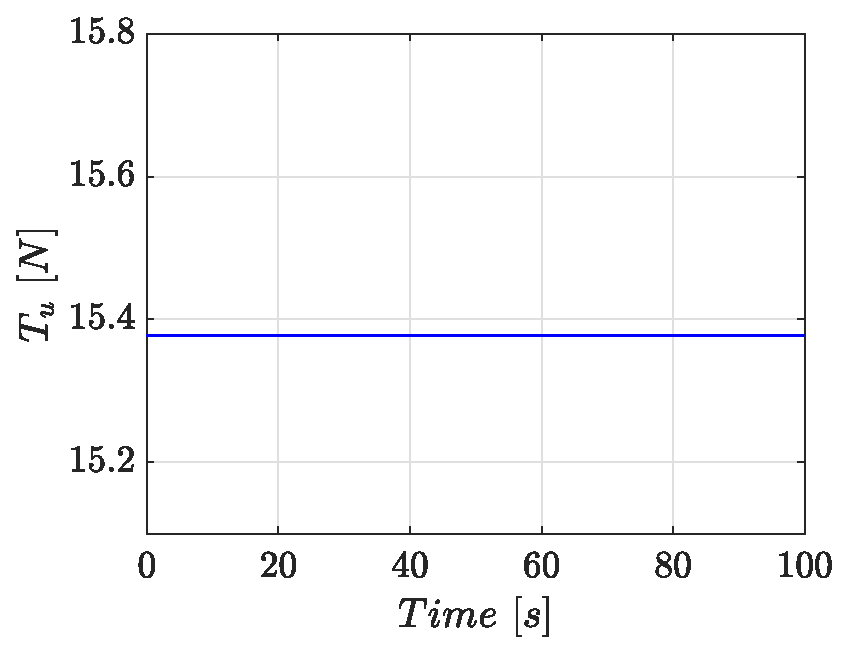
\includegraphics[width=7.0cm]{stabilize_u_h_imp}
\caption{Thrust}
\label{fig:stabilize_u_h_imp}
\end{subfigure}%
\begin{subfigure}{.5\linewidth}
\centering
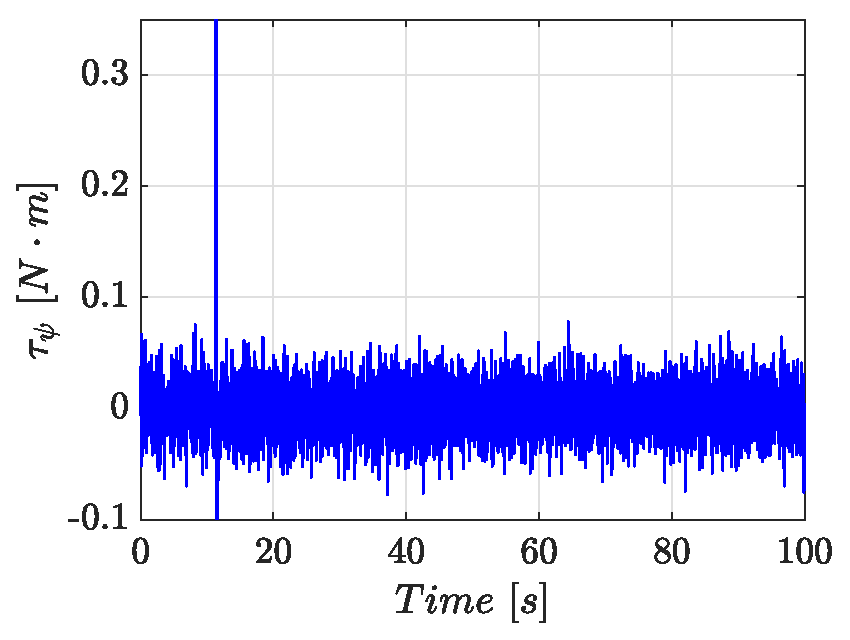
\includegraphics[width=7.0cm]{stabilize_taupsi_h_imp}
\caption{Yaw torque}
\label{fig:stabilize_taupsi_h_imp}
\end{subfigure}\\[1ex]
\begin{subfigure}{0.5\linewidth}
\centering
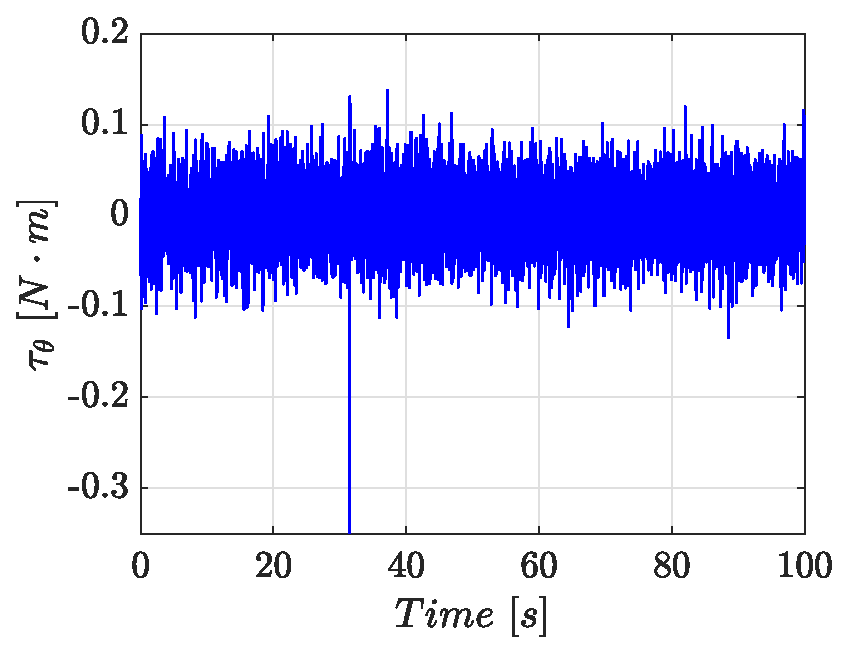
\includegraphics[width=7.0cm]{stabilize_tautheta_h_imp}
\caption{Roll torque}
\label{fig:stabilize_tautheta_h_imp}
\end{subfigure}
\begin{subfigure}{0.5\linewidth}
\centering
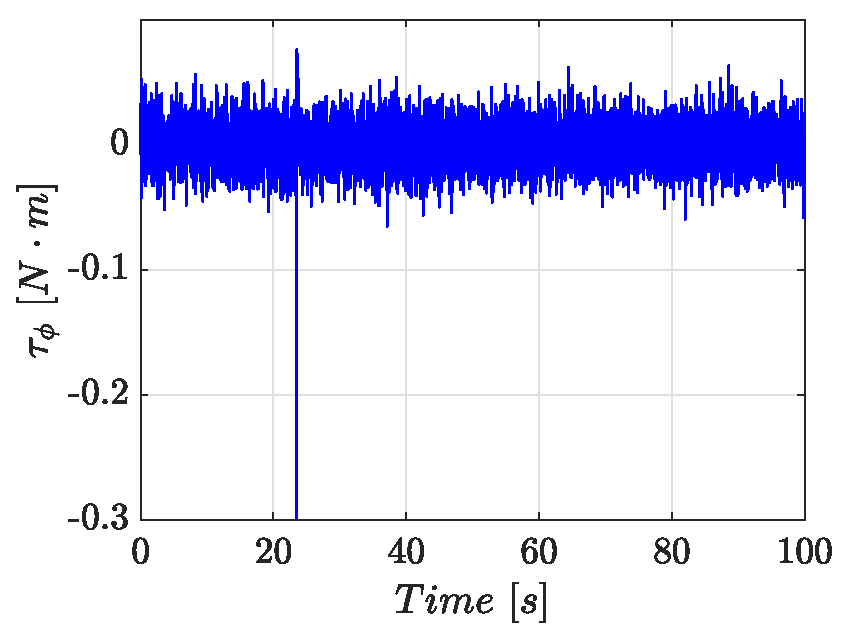
\includegraphics[width=7.0cm]{stabilize_tauphi_h_imp}
\caption{Pitch torque}
\label{fig:stabilize_tauphi_h_imp}
\end{subfigure}
\caption{Control signals in $H_\infty$ control test for stabilize mode}
\label{fig:stabilize_control_h}
\end{figure}

\begin{figure}[H]
\begin{subfigure}{.5\linewidth}
\centering
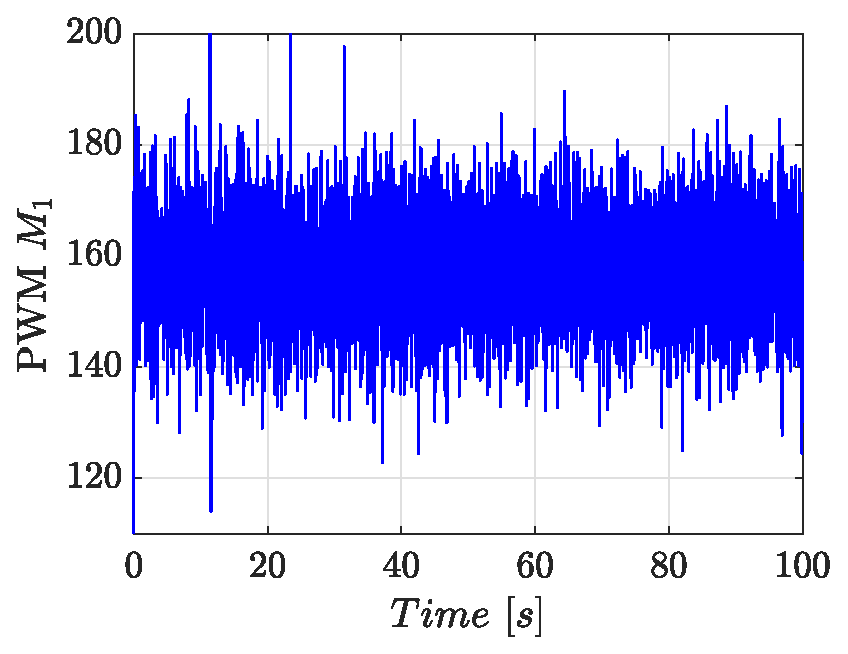
\includegraphics[width=7.0cm]{stabilize_pwm1_h_imp}
\caption{\textit{PWM} signal in Motor $M_1$}
\label{fig:stabilize_pwm_h_imp}
\end{subfigure}%
\begin{subfigure}{.5\linewidth}
\centering
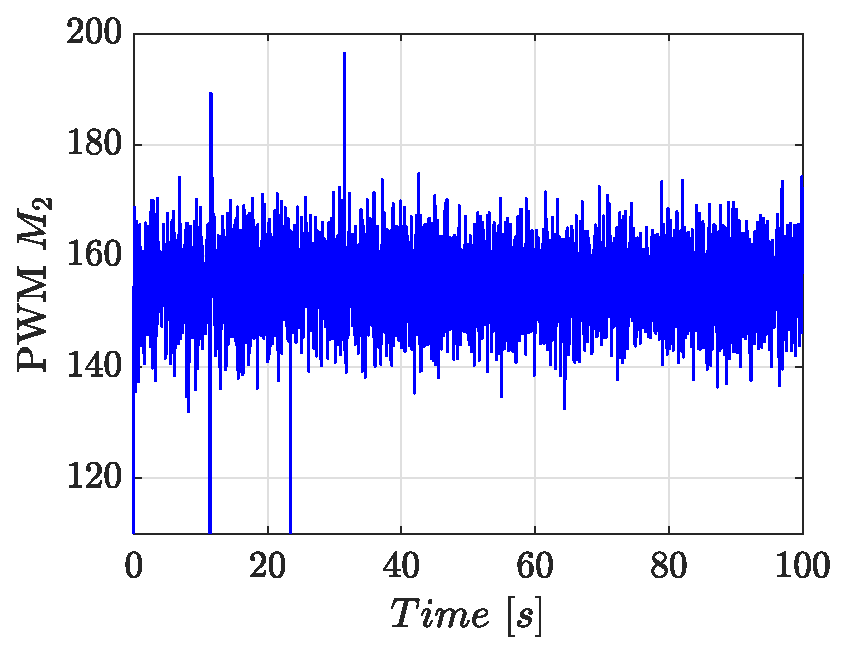
\includegraphics[width=7.0cm]{stabilize_pwm2_h_imp}
\caption{\textit{PWM} signal in Motor $M_2$}
\label{fig:stabilize_pwm2_h_imp}
\end{subfigure}\\[1ex]
\begin{subfigure}{0.5\linewidth}
\centering
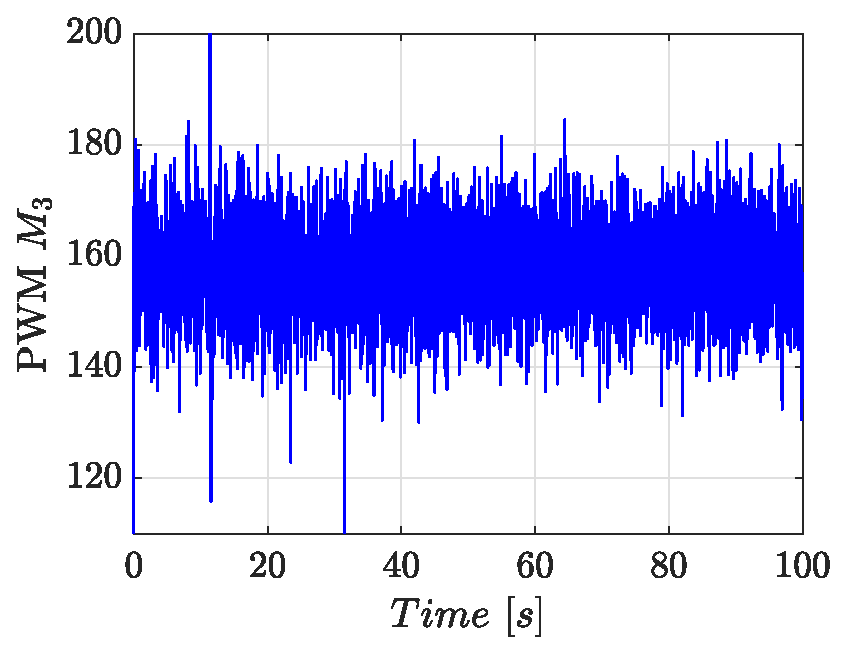
\includegraphics[width=7.0cm]{stabilize_pwm3_h_imp}
\caption{\textit{PWM} signal in Motor $M_3$}
\label{fig:stabilize_pwm3_h_imp}
\end{subfigure}
\begin{subfigure}{0.5\linewidth}
\centering
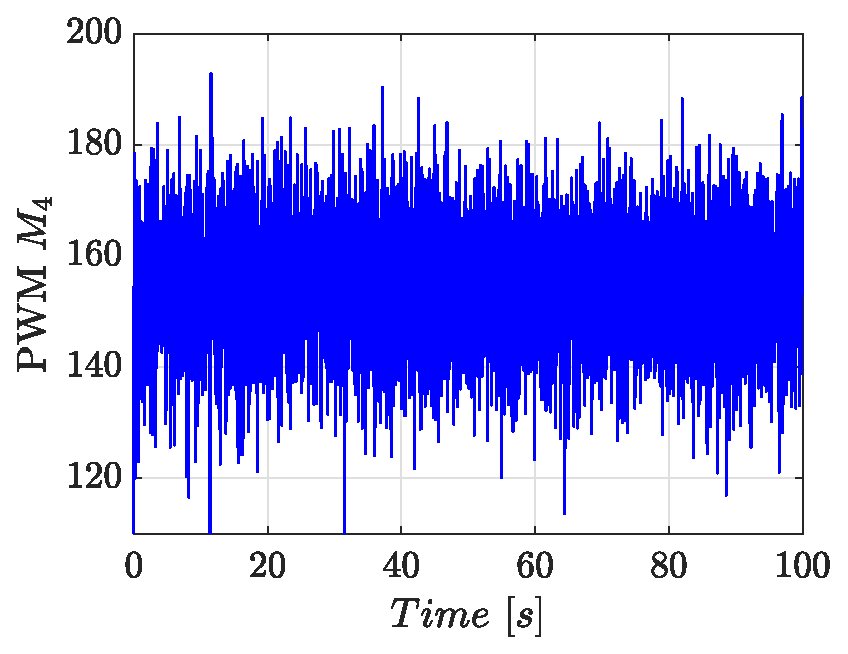
\includegraphics[width=7.0cm]{stabilize_pwm4_h_imp}
\caption{\textit{PWM} signal in Motor $M_4$}
\label{fig:stabilize_pwm4_h_imp}
\end{subfigure}
\caption{\textit{PWM} signals in $H_\infty$ control test for stabilize mode}
\label{fig:stabilize_pwm_h}
\end{figure}


\section*{Altitude Hold Mode}
\subsection*{LQI Controller}
\begin{figure}[H]
\begin{subfigure}{.5\linewidth}
\centering
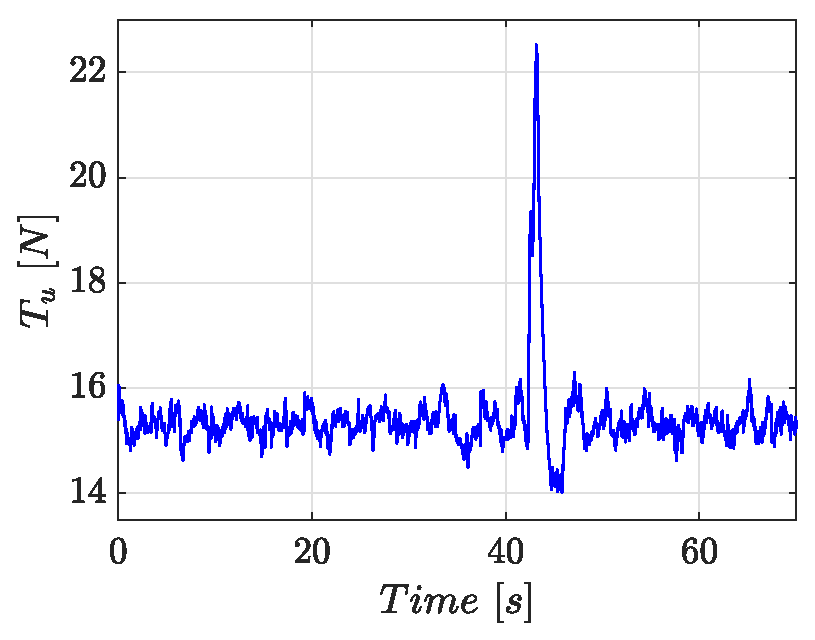
\includegraphics[width=7.0cm]{althold_u_lqi_imp}
\caption{Thrust}
\label{fig:althold_u_lqi_imp}
\end{subfigure}%
\begin{subfigure}{.5\linewidth}
\centering
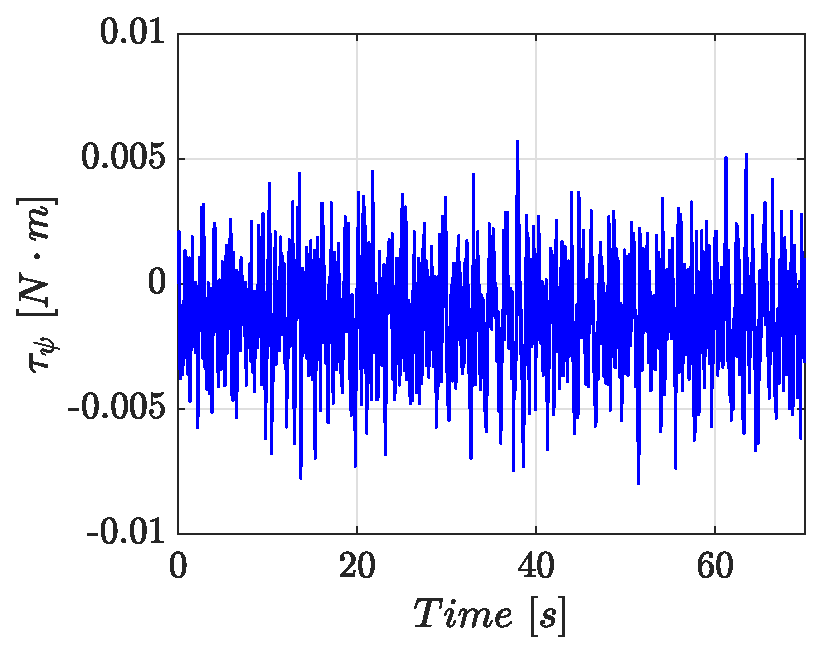
\includegraphics[width=7.0cm]{althold_taupsi_lqi_imp}
\caption{Yaw torque}
\label{fig:althold_taupsi_lqi_imp}
\end{subfigure}\\[1ex]
\begin{subfigure}{0.5\linewidth}
\centering
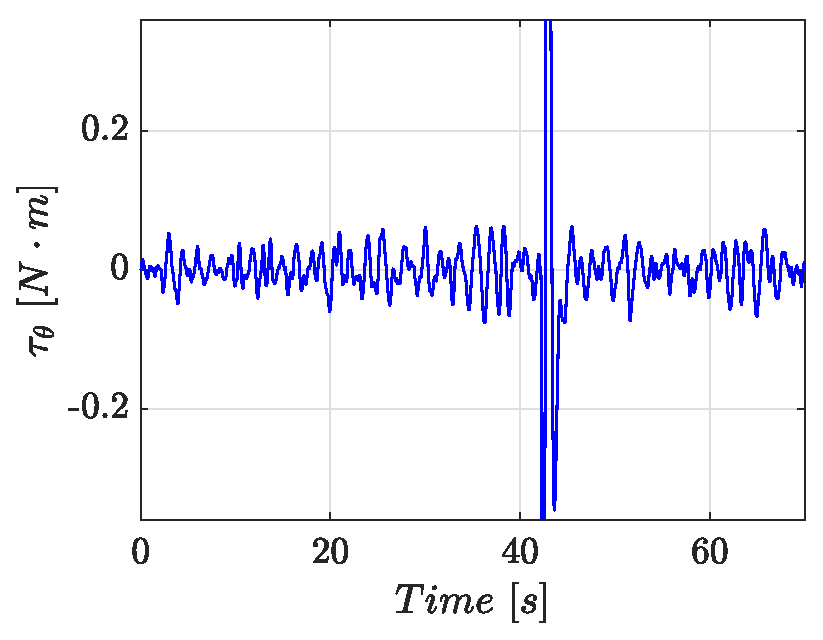
\includegraphics[width=7.0cm]{althold_tautheta_lqi_imp}
\caption{Roll torque}
\label{fig:althold_tautheta_lqi_imp}
\end{subfigure}
\begin{subfigure}{0.5\linewidth}
\centering
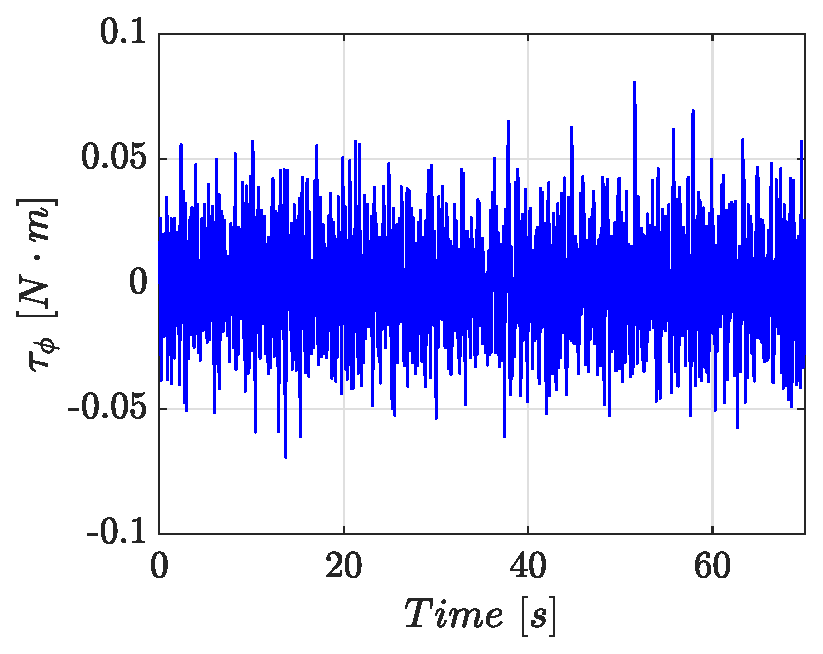
\includegraphics[width=7.0cm]{althold_tauphi_lqi_imp}
\caption{Pitch torque}
\label{fig:althold_tauphi_lqi_imp}
\end{subfigure}
\caption{Control signals in LQI control test for altitude hold mode}
\label{fig:althold_control_lqi}
\end{figure}

\begin{figure}[H]
\begin{subfigure}{.5\linewidth}
\centering
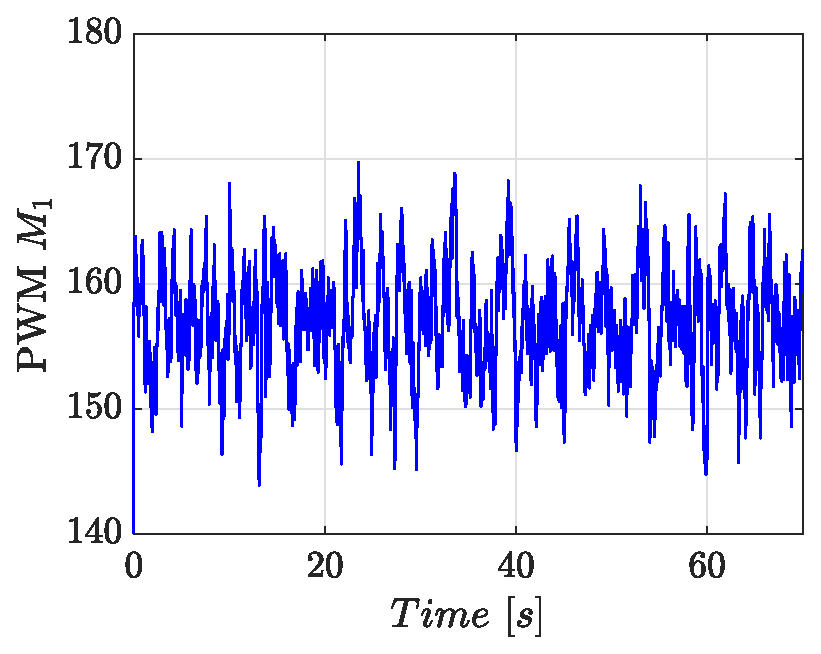
\includegraphics[width=7.0cm]{althold_pwm1_lqi_imp}
\caption{\textit{PWM} signal in Motor $M_1$}
\label{fig:althold_pwm_lqi_imp}
\end{subfigure}%
\begin{subfigure}{.5\linewidth}
\centering
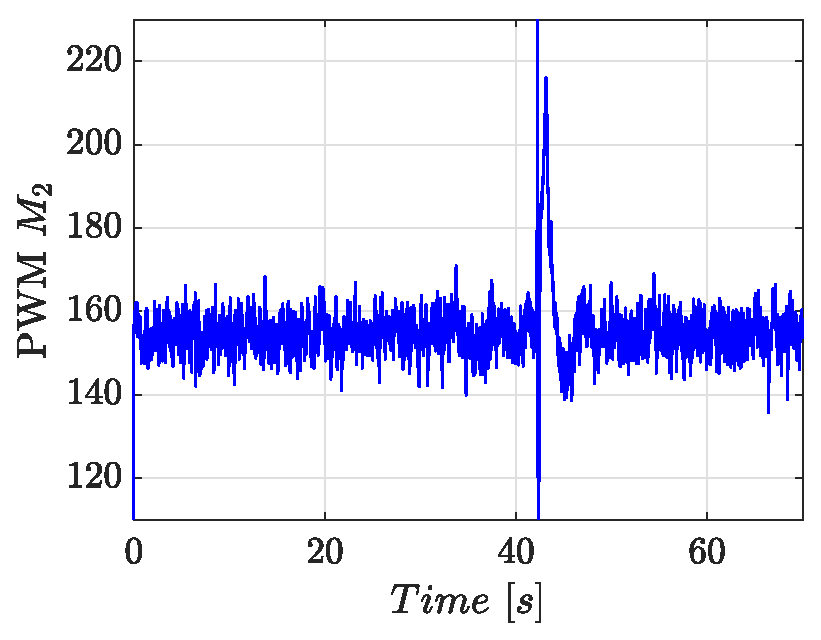
\includegraphics[width=7.0cm]{althold_pwm2_lqi_imp}
\caption{\textit{PWM} signal in Motor $M_2$}
\label{fig:althold_pwm2_lqi_imp}
\end{subfigure}\\[1ex]
\begin{subfigure}{0.5\linewidth}
\centering
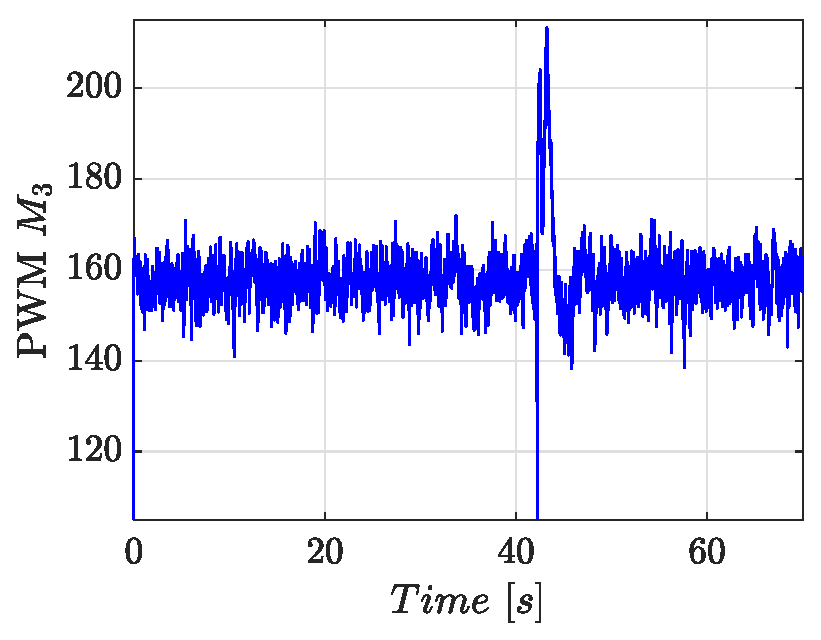
\includegraphics[width=7.0cm]{althold_pwm3_lqi_imp}
\caption{\textit{PWM} signal in Motor $M_3$}
\label{fig:althold_pwm3_lqi_imp}
\end{subfigure}
\begin{subfigure}{0.5\linewidth}
\centering
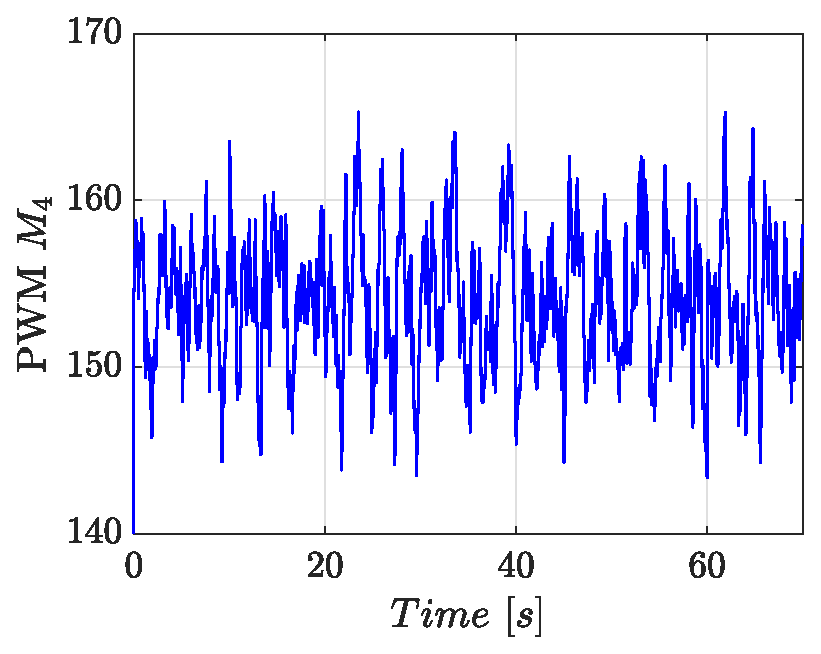
\includegraphics[width=7.0cm]{althold_pwm4_lqi_imp}
\caption{\textit{PWM} signal in Motor $M_4$}
\label{fig:althold_pwm4_lqi_imp}
\end{subfigure}
\caption{\textit{PWM} signals in LQI control test for altitude hold mode}
\label{fig:althold_pwm_lqi}
\end{figure}

\subsection*{$H_\infty$ Controller}

\begin{figure}[H]
\begin{subfigure}{.5\linewidth}
\centering
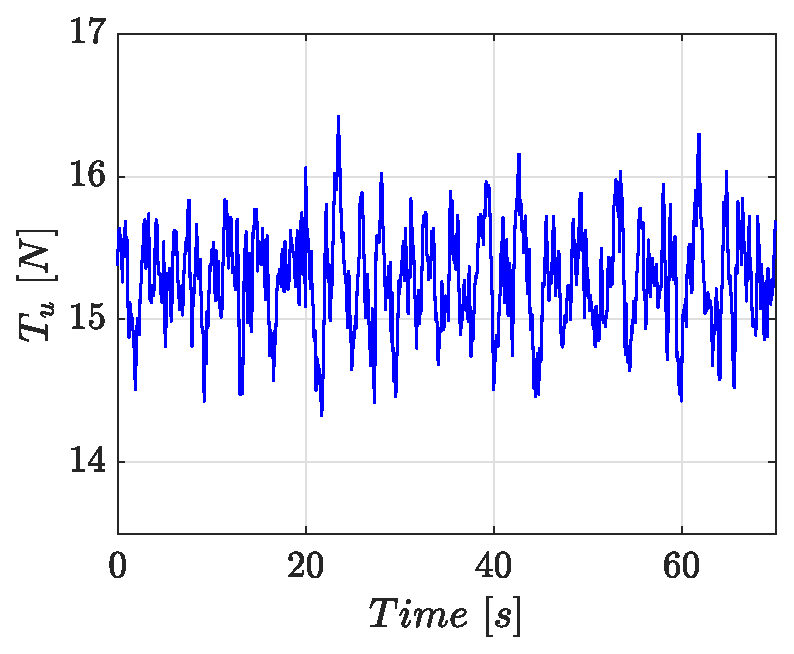
\includegraphics[width=7.0cm]{althold_u_h_imp}
\caption{Thrust}
\label{fig:althold_u_h_imp}
\end{subfigure}%
\begin{subfigure}{.5\linewidth}
\centering
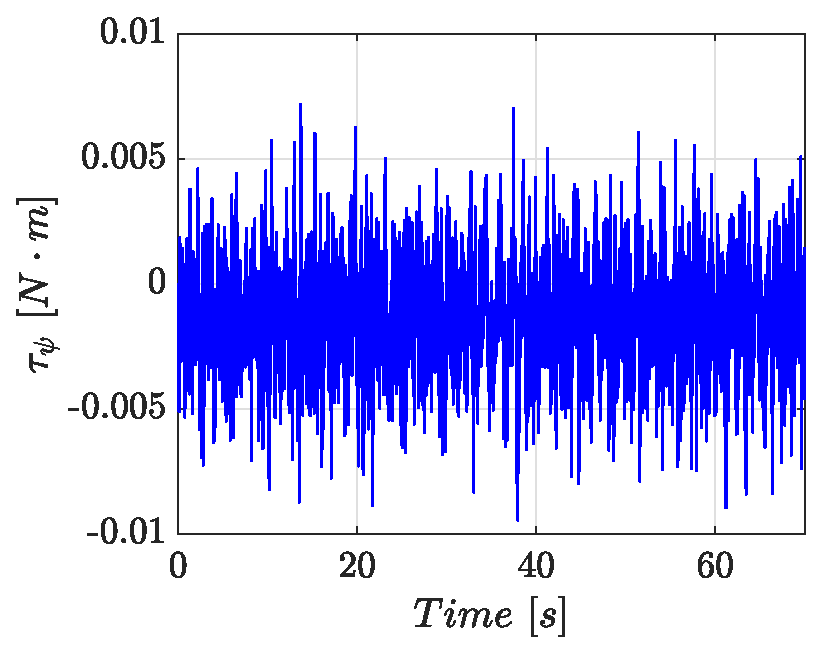
\includegraphics[width=7.0cm]{althold_taupsi_h_imp}
\caption{Yaw torque}
\label{fig:althold_taupsi_h_imp}
\end{subfigure}\\[1ex]
\begin{subfigure}{0.5\linewidth}
\centering
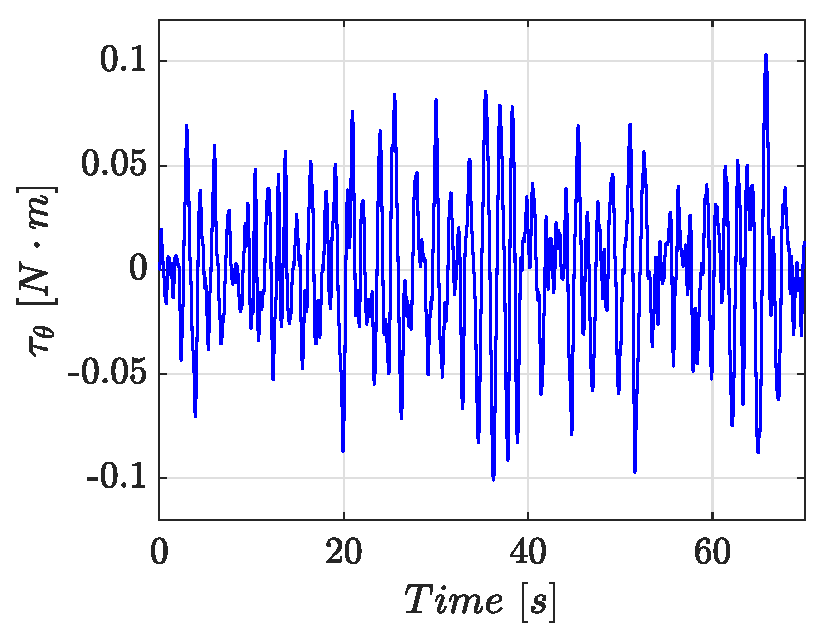
\includegraphics[width=7.0cm]{althold_tautheta_h_imp}
\caption{Roll torque}
\label{fig:althold_tautheta_h_imp}
\end{subfigure}
\begin{subfigure}{0.5\linewidth}
\centering
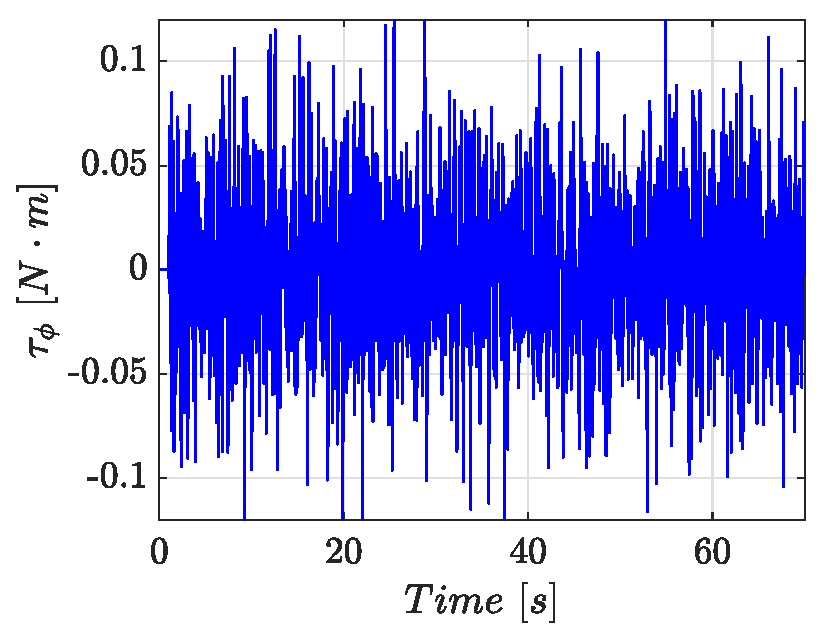
\includegraphics[width=7.0cm]{althold_tauphi_h_imp}
\caption{Pitch torque}
\label{fig:althold_tauphi_h_imp}
\end{subfigure}
\caption{Control signals in $H_\infty$ control test for altitude hold mode}
\label{fig:althold_control_h}
\end{figure}

\begin{figure}[H]
\begin{subfigure}{.5\linewidth}
\centering
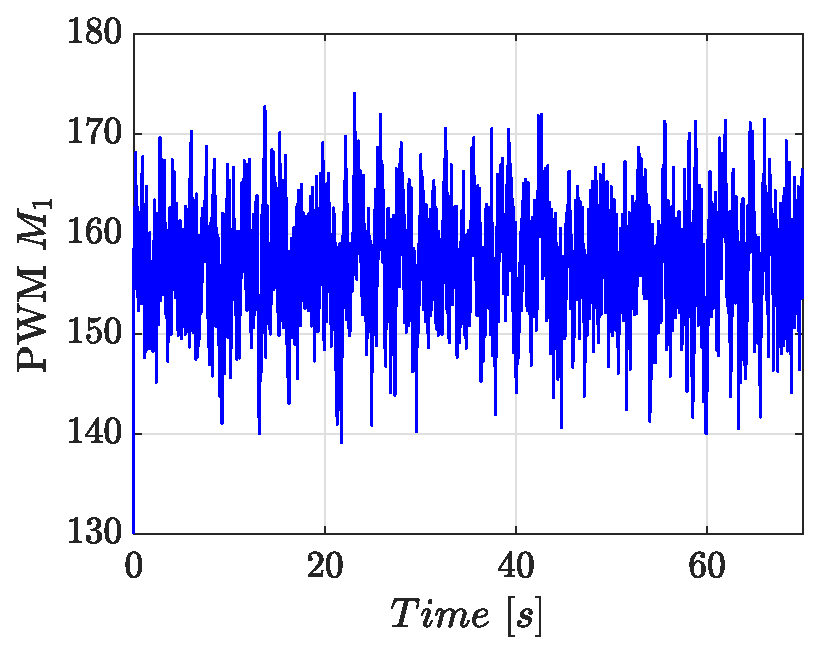
\includegraphics[width=7.0cm]{althold_pwm1_h_imp}
\caption{\textit{PWM} signal in Motor $M_1$}
\label{fig:althold_pwm_h_imp}
\end{subfigure}%
\begin{subfigure}{.5\linewidth}
\centering
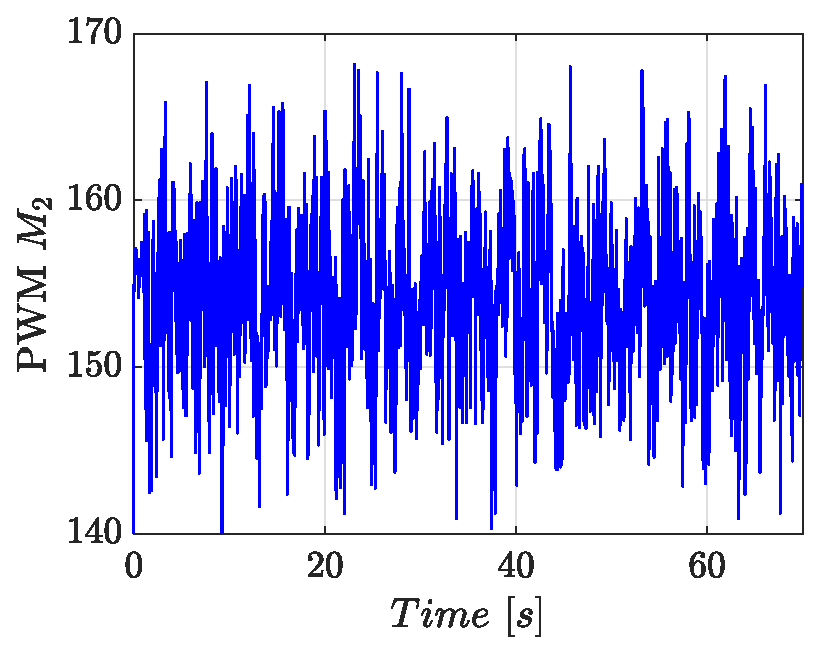
\includegraphics[width=7.0cm]{althold_pwm2_h_imp}
\caption{\textit{PWM} signal in Motor $M_2$}
\label{fig:althold_pwm2_h_imp}
\end{subfigure}\\[1ex]
\begin{subfigure}{0.5\linewidth}
\centering
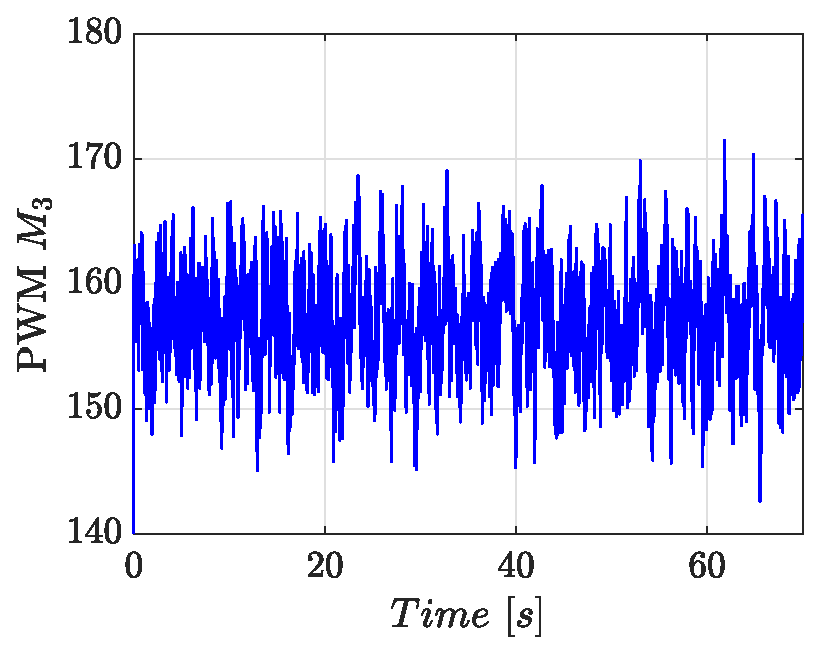
\includegraphics[width=7.0cm]{althold_pwm3_h_imp}
\caption{\textit{PWM} signal in Motor $M_3$}
\label{fig:althold_pwm3_h_imp}
\end{subfigure}
\begin{subfigure}{0.5\linewidth}
\centering
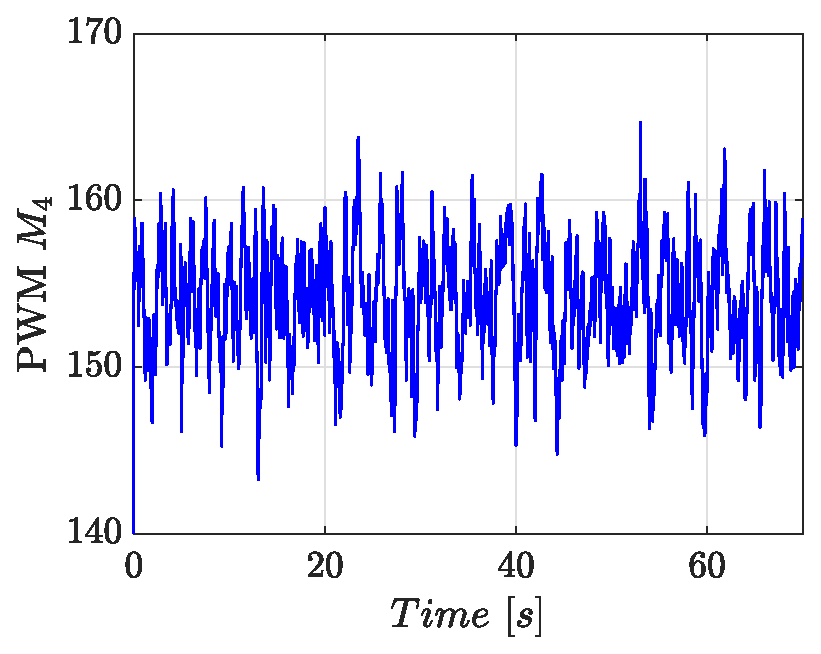
\includegraphics[width=7.0cm]{althold_pwm4_h_imp}
\caption{\textit{PWM} signal in Motor $M_4$}
\label{fig:althold_pwm4_h_imp}
\end{subfigure}
\caption{\textit{PWM} signals in $H_\infty$ control test for altitude hold mode}
\label{fig:althold_pwm_h}
\end{figure}

\section*{GNSS-Dependent Mode}

\subsection*{LQI Controller}

\begin{figure}[H]
\begin{subfigure}{.5\linewidth}
\centering
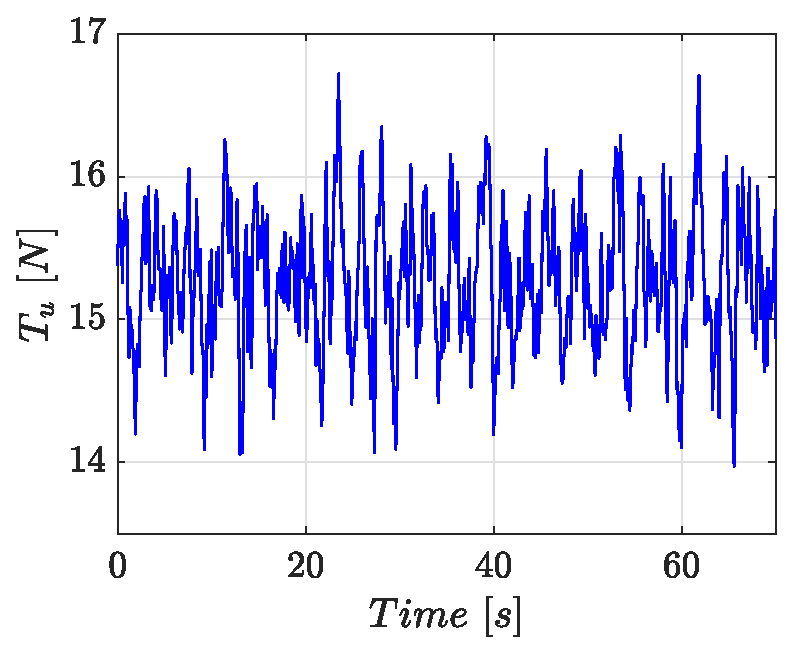
\includegraphics[width=7.0cm]{auto_u_lqi_imp}
\caption{Thrust}
\label{fig:auto_u_lqi_imp}
\end{subfigure}%
\begin{subfigure}{.5\linewidth}
\centering
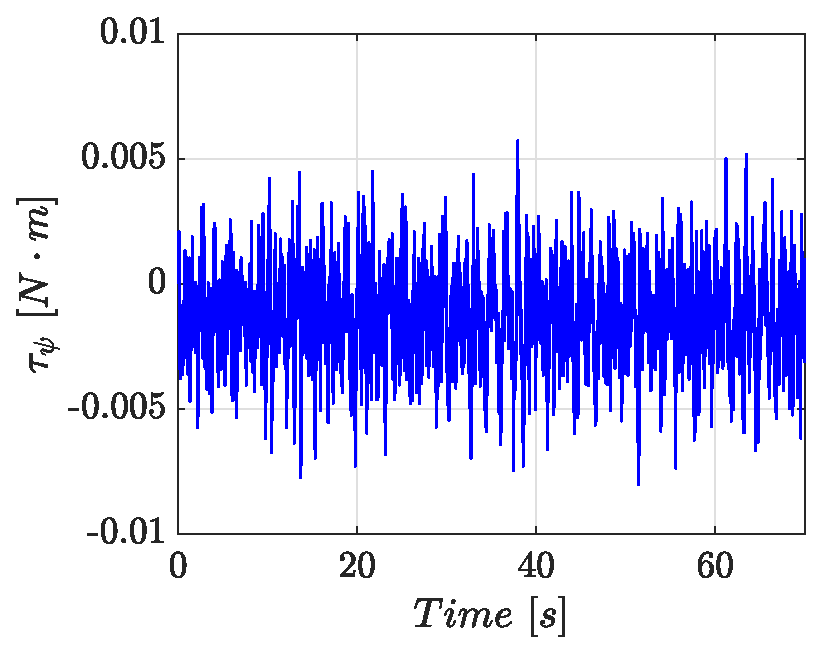
\includegraphics[width=7.0cm]{auto_taupsi_lqi_imp}
\caption{Yaw torque}
\label{fig:auto_taupsi_lqi_imp}
\end{subfigure}\\[1ex]
\begin{subfigure}{0.5\linewidth}
\centering
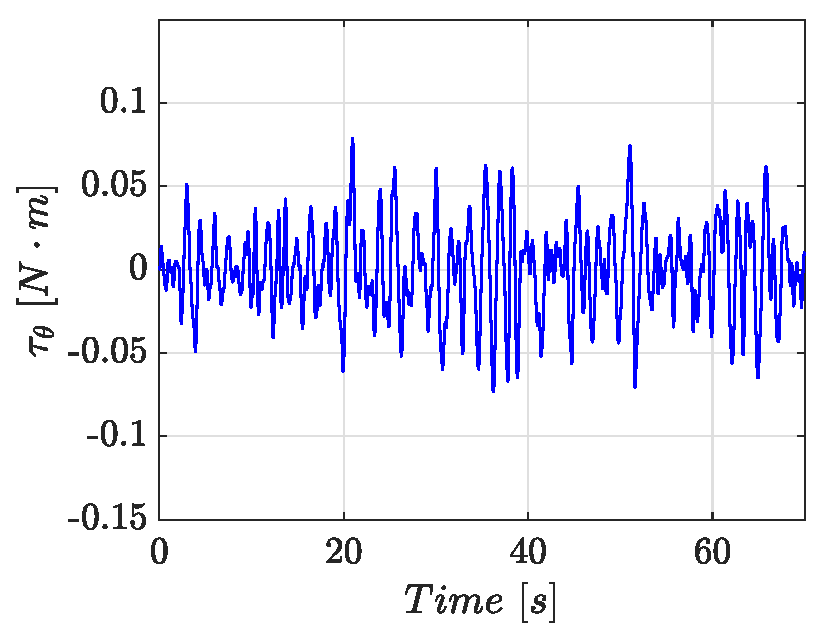
\includegraphics[width=7.0cm]{auto_tautheta_lqi_imp}
\caption{Roll torque}
\label{fig:auto_tautheta_lqi_imp}
\end{subfigure}
\begin{subfigure}{0.5\linewidth}
\centering
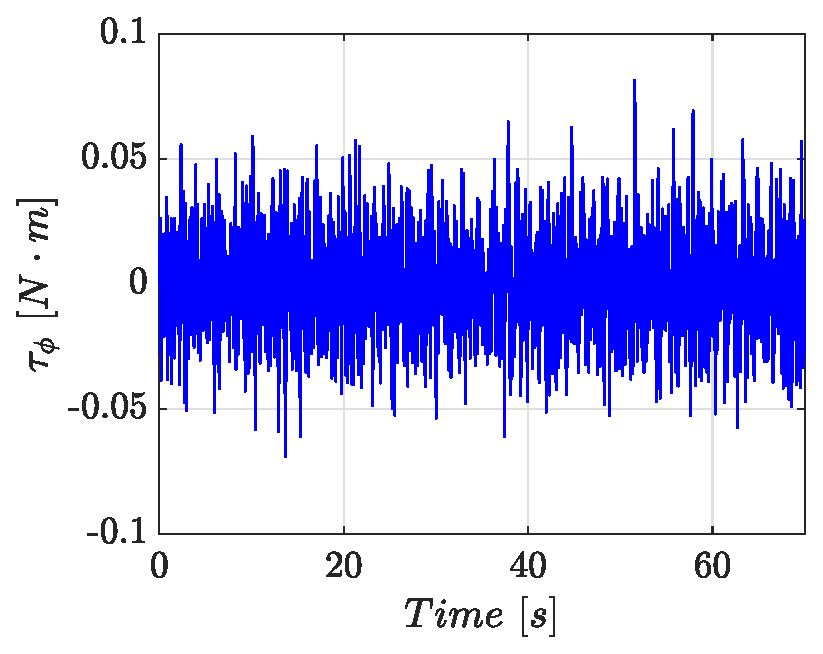
\includegraphics[width=7.0cm]{auto_tauphi_lqi_imp}
\caption{Pitch torque}
\label{fig:auto_tauphi_h_lqi}
\end{subfigure}
\caption{Control signals in LQI control test for GNSS-Dependent modes}
\label{fig:auto_control_lqi}
\end{figure}

\begin{figure}[H]
\begin{subfigure}{.5\linewidth}
\centering
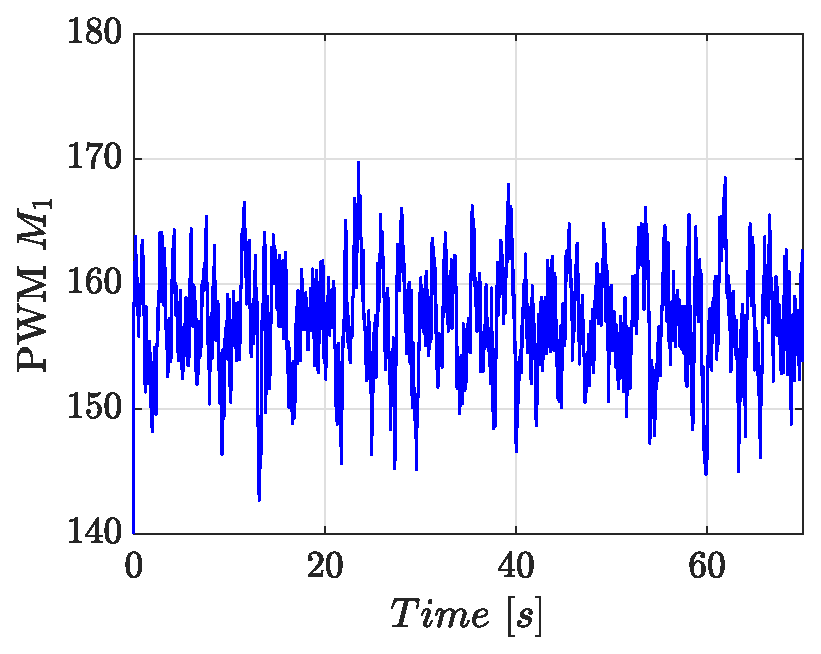
\includegraphics[width=7.0cm]{auto_pwm1_lqi_imp}
\caption{\textit{PWM} signal in Motor $M_1$}
\label{fig:auto_pwm_lqi_imp}
\end{subfigure}%
\begin{subfigure}{.5\linewidth}
\centering
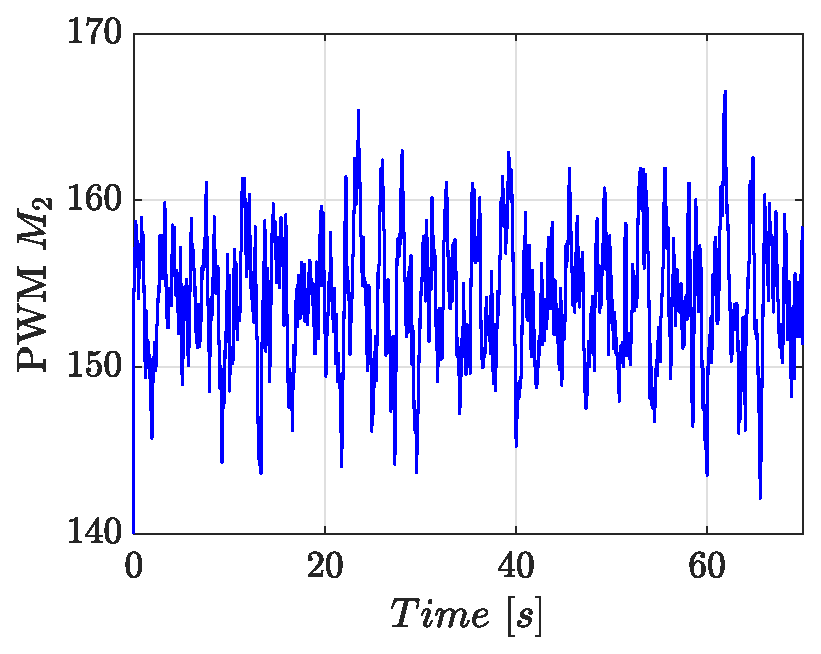
\includegraphics[width=7.0cm]{auto_pwm2_lqi_imp}
\caption{\textit{PWM} signal in Motor $M_2$}
\label{fig:auto_pwm2_lqi_imp}
\end{subfigure}\\[1ex]
\begin{subfigure}{0.5\linewidth}
\centering
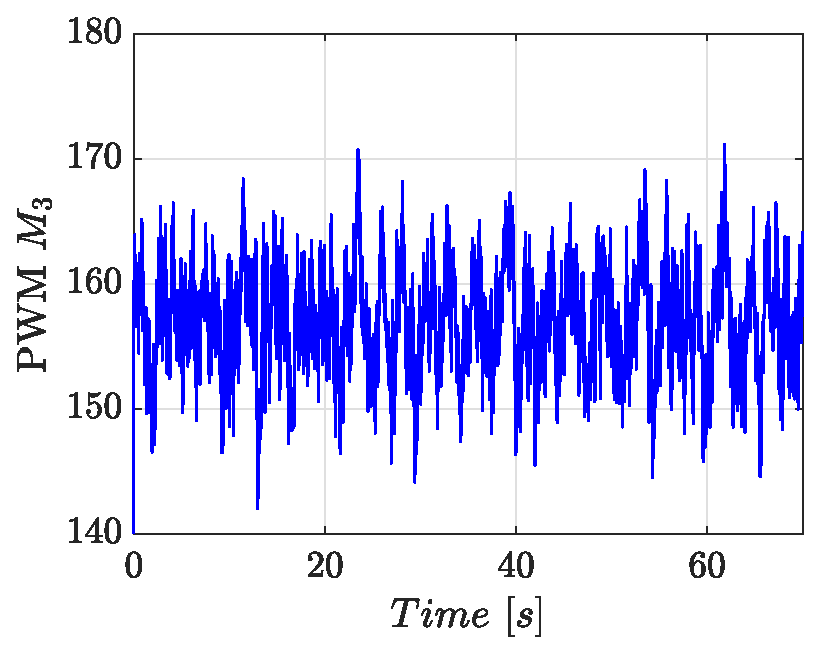
\includegraphics[width=7.0cm]{auto_pwm3_lqi_imp}
\caption{\textit{PWM} signal in Motor $M_3$}
\label{fig:auto_pwm3_lqi_imp}
\end{subfigure}
\begin{subfigure}{0.5\linewidth}
\centering
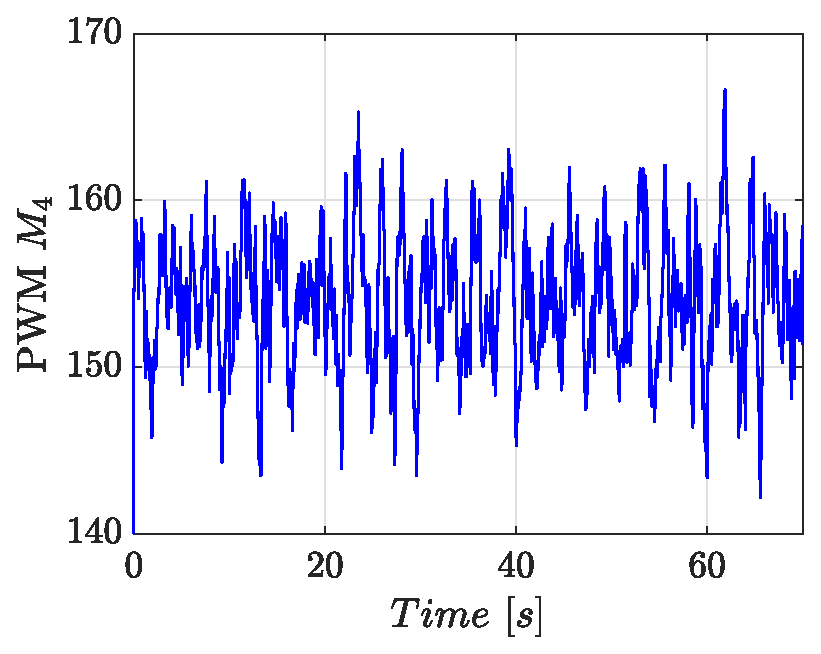
\includegraphics[width=7.0cm]{auto_pwm4_lqi_imp}
\caption{\textit{PWM} signal in Motor $M_4$}
\label{fig:auto_pwm4_lqi_imp}
\end{subfigure}
\caption{\textit{PWM} signals in LQI control test for GNSS-Dependent modes}
\label{fig:auto_pwm_lqi}
\end{figure}



\subsection*{$H_\infty$ Controller}

\begin{figure}[H]
\begin{subfigure}{.5\linewidth}
\centering
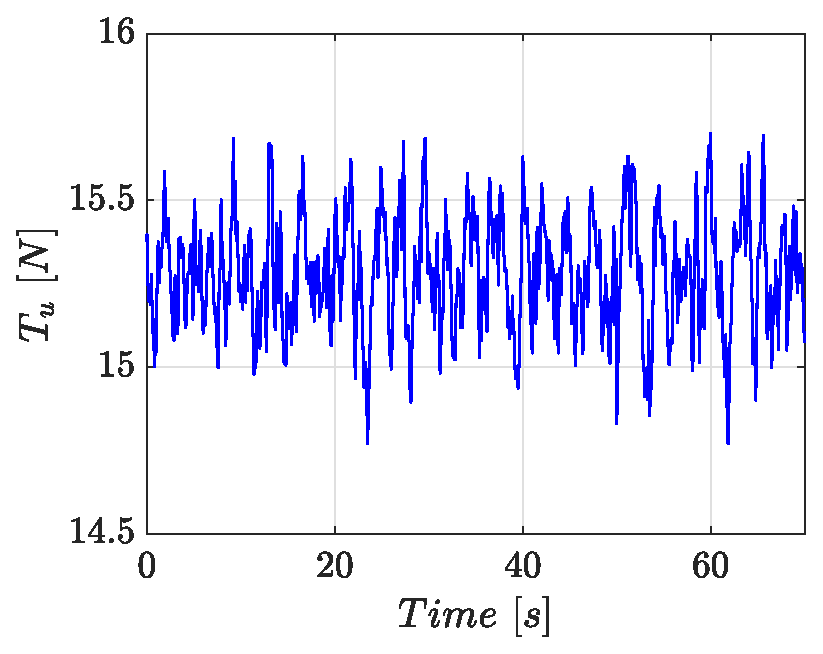
\includegraphics[width=7.0cm]{auto_u_h_imp}
\caption{Thrust}
\label{fig:auto_u_h_imp}
\end{subfigure}%
\begin{subfigure}{.5\linewidth}
\centering
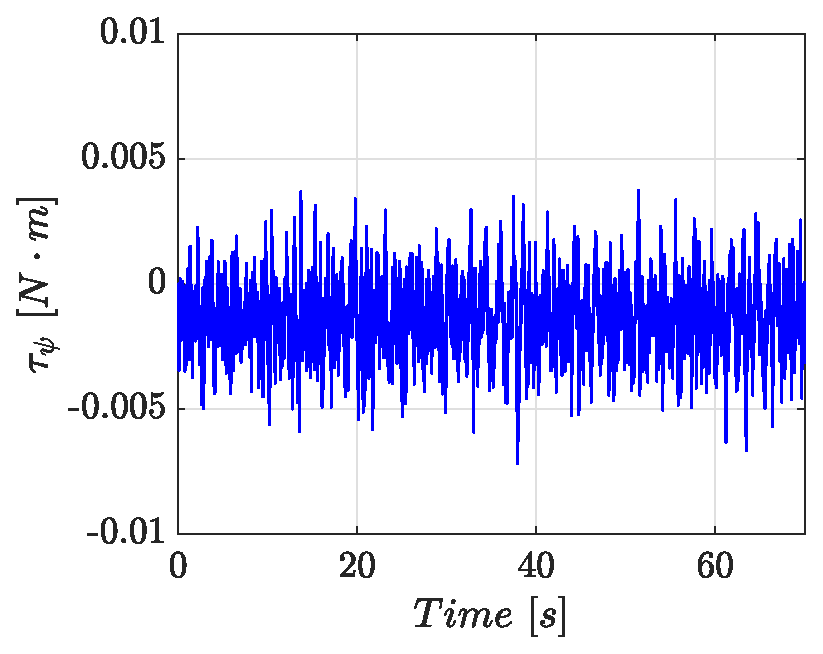
\includegraphics[width=7.0cm]{auto_taupsi_h_imp}
\caption{Yaw torque}
\label{fig:auto_taupsi_h_imp}
\end{subfigure}\\[1ex]
\begin{subfigure}{0.5\linewidth}
\centering
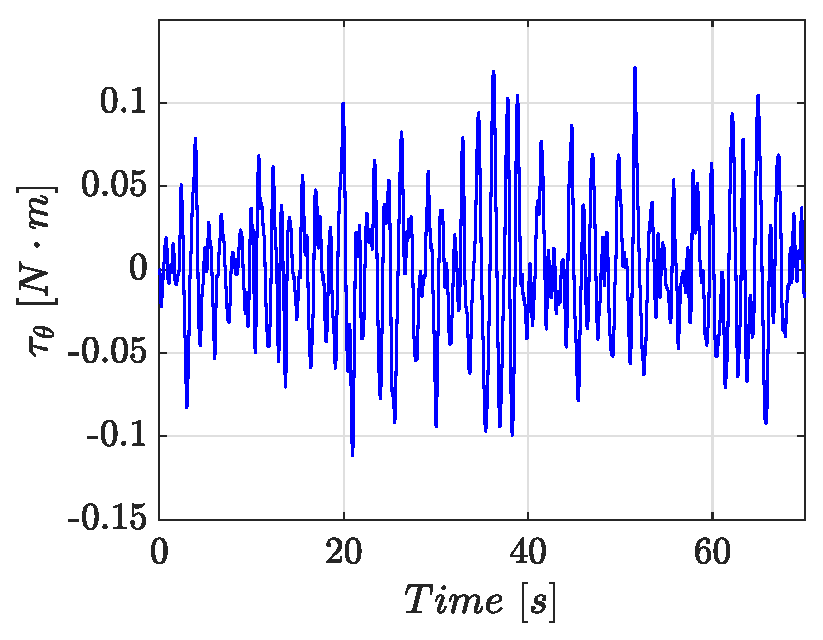
\includegraphics[width=7.0cm]{auto_tautheta_h_imp}
\caption{Roll torque}
\label{fig:auto_tautheta_h_imp}
\end{subfigure}
\begin{subfigure}{0.5\linewidth}
\centering
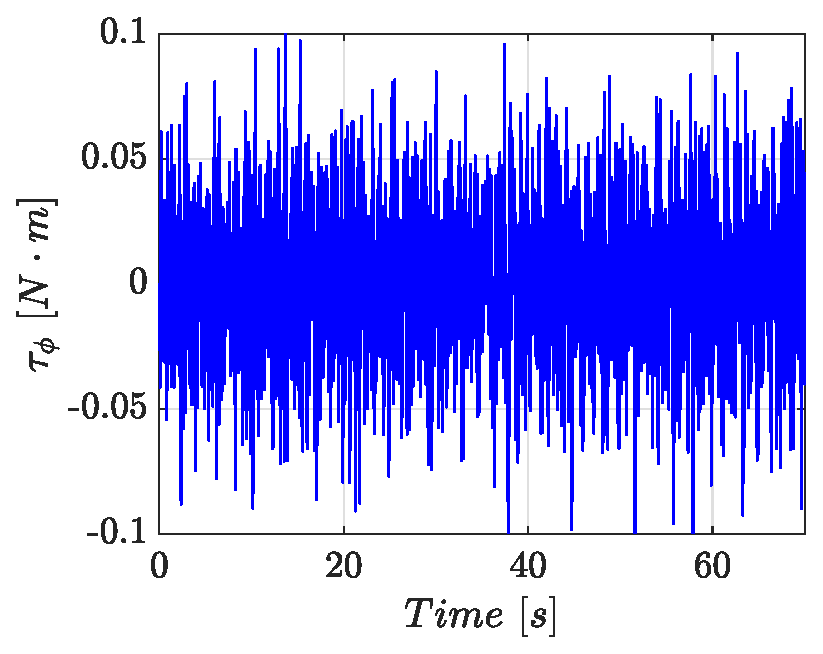
\includegraphics[width=7.0cm]{auto_tauphi_h_imp}
\caption{Pitch torque}
\label{fig:auto_tauphi_h_imp}
\end{subfigure}
\caption{Control signals in $H_\infty$ control test for GNSS-Dependent modes}
\label{fig:auto_control_h}
\end{figure}

\begin{figure}[H]
\begin{subfigure}{.5\linewidth}
\centering
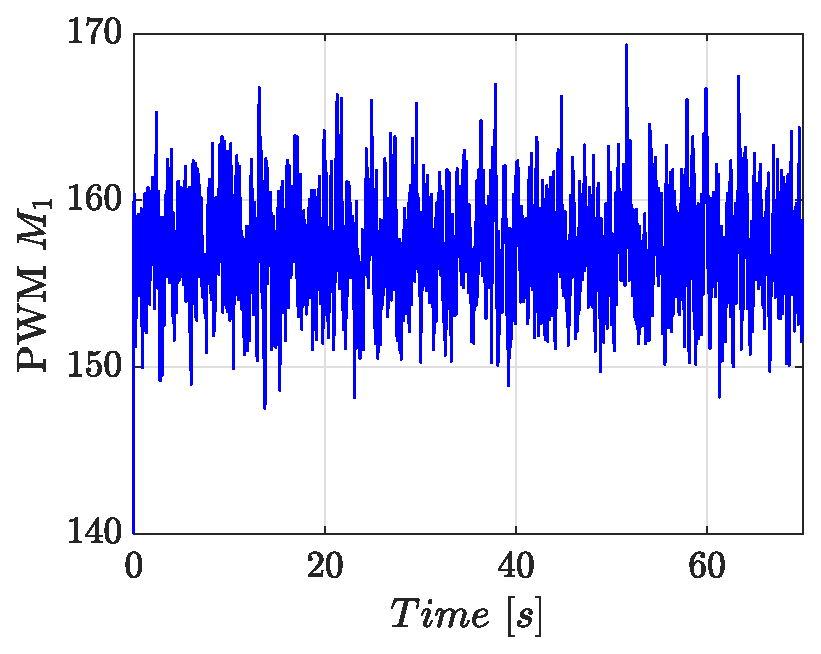
\includegraphics[width=7.0cm]{auto_pwm1_h_imp}
\caption{\textit{PWM} signal in Motor $M_1$}
\label{fig:auto_pwm_h_imp}
\end{subfigure}%
\begin{subfigure}{.5\linewidth}
\centering
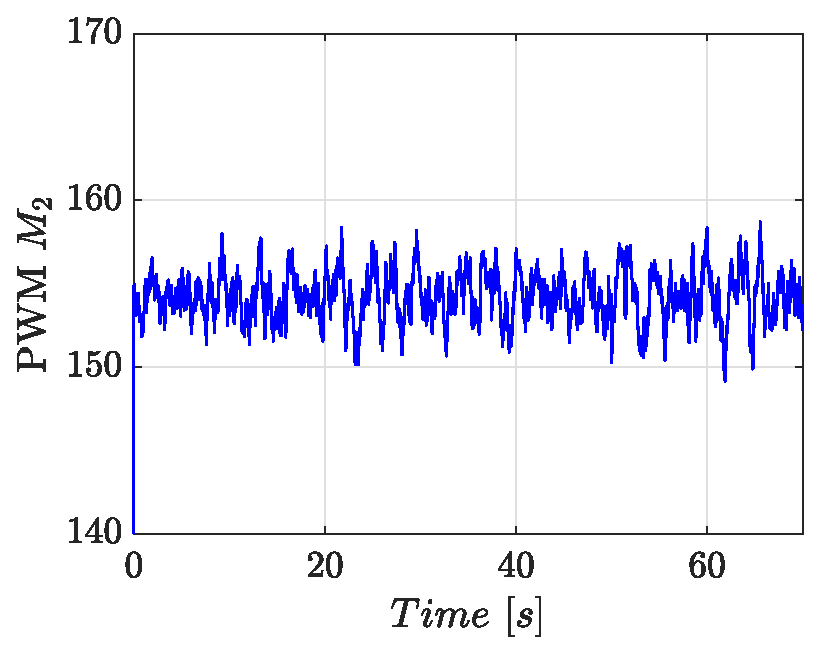
\includegraphics[width=7.0cm]{auto_pwm2_h_imp}
\caption{\textit{PWM} signal in Motor $M_2$}
\label{fig:auto_pwm2_h_imp}
\end{subfigure}\\[1ex]
\begin{subfigure}{0.5\linewidth}
\centering
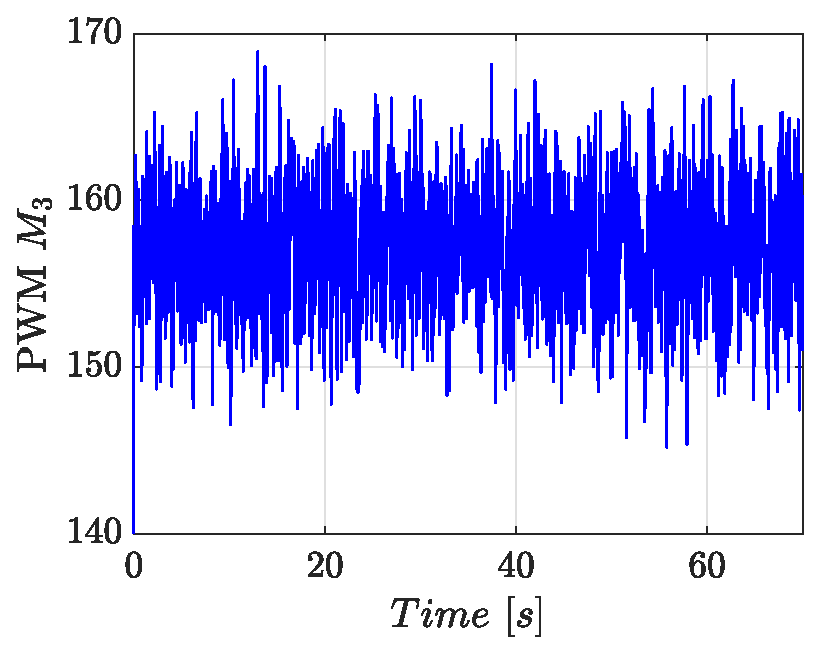
\includegraphics[width=7.0cm]{auto_pwm3_h_imp}
\caption{\textit{PWM} signal in Motor $M_3$}
\label{fig:auto_pwm3_h_imp}
\end{subfigure}
\begin{subfigure}{0.5\linewidth}
\centering
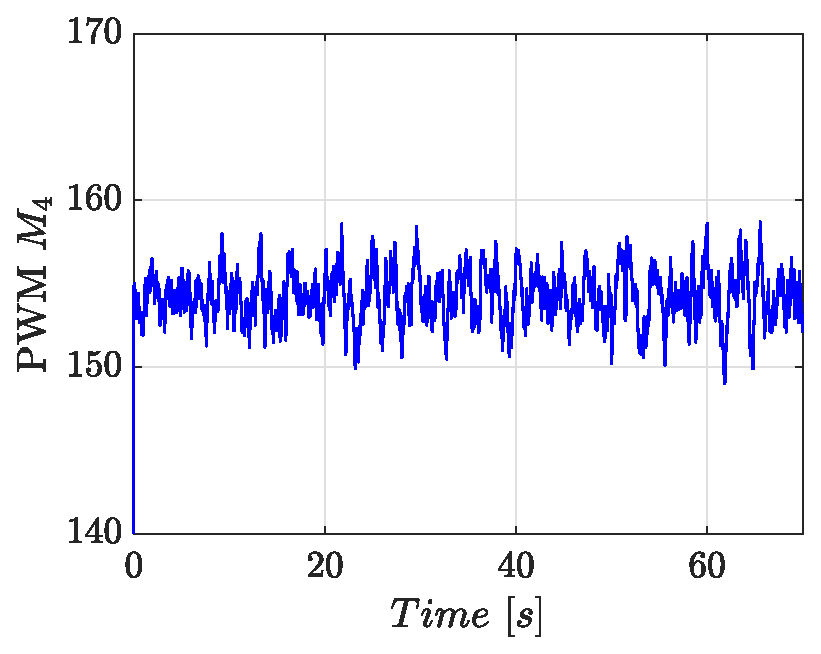
\includegraphics[width=7.0cm]{auto_pwm4_h_imp}
\caption{\textit{PWM} signal in Motor $M_4$}
\label{fig:auto_pwm4_h_imp}
\end{subfigure}
\caption{\textit{PWM} signals in $H_\infty$ control test for GNSS-Dependent modes}
\label{fig:auto_pwm_h}
\end{figure}



\end{appendices}